%! Author = tstreule

\section{Optical Biosensors}
%%%%%%%%%%%%%%%%%%%%%%%%%%%%%%%%%%%%%%%%%%%%%%%%%%%%%%
%%%%%%%%%%%%%%%%%%%%%%%%%%%%%%%%%%%%%%%%%%%%%%%%%%%%%%
%	\subsection{Optical Methods}
%	%
%	\begin{itemize}
%		\item \underline{Reflection based} (ELM, SAR)\\
%			information through $\Delta\phi$ and $\Delta$amplitude
%		\item \underline{Interference based} (OIA, TINS)\\
%			information through color change \quad
%			very sensitive to $\Delta$thickness
%		\item \underline{Evanescent field} techniques (\textbf{SPR}, \textbf{OWLS}, RM, FTIR, SAR)\\
%			information through $\Delta n$ ($n$: refractive index)
%	\end{itemize}
%%%%%%%%%%%%%%%%%%%%%%%%%%%%%%%%%%%%%%%%%%%%%%%%%%%%%%
\subsection{EM}
%
\textbf{Relations}:\\
$c_0 = \frac{1}{\sqrt{\epsilon_0\mu_0}}$ \hfill
$k_0 = \frac{2\pi}{\lambda_0} = \frac{\omega}{c_0} = \omega\sqrt{\epsilon_0\mu_0}$ \hfill
$k = \frac{2\pi n}{\lambda}$ \hfill
$n = \frac{c_0}{c} = \sqrt{\epsilon_r\mu_r} \simeq \sqrt{\epsilon_r}$
\formula{Dispersion relation}{k^2 = \epsilon\omega^2 = \epsilon k_0^2c_0^2 = k_0\frac{\epsilon}{\epsilon_0} = k_0^2\epsilon_r = (k_0n)^2}

\formbox{\textbf{Plane waves}}{\vec{E}(\vec{r},t) = \vec{E}_0\;\eu^{\iu(\vec{k}\vec{r}-\omega t)}} \\
whereby \hfill
$\partial_t \hat= -\iu\omega$, \hfill
$\partial_x \hat= \iu k_x$, \hfill
$\partial_z \hat= \iu k_z$, \hfill
$\partial_y \hat= 0$ (infinite extent)
\formula{Depth of penetration}{d_p = \frac{\lambda}{4\pi} \frac{1}{\sqrt{n\ped{inc}^2\sin^2\theta -n_2^2}}}
\quad (about $\unit[500]{nm}$)
%%%%%%%%%%%%%%%%%%%%%%%%%%%%%%%%%%%%%%%%%%%%%%%%%%%%%%
\subsection{Evanescent Field Techniques}
%
\formtex{\textit{Recap}}{Always \textbf{total reflection} for $n\ped{inc}>n_2$}
\formtex{Evanescence}{Negligible change of sensitivity compared to}
\formtex{~}{the size of the antibodies}
%%%%%%%%%%%%%%%%%%%%%%%%%%%%%%%%%%%%%%%%%%%%%%%%%%%%%%
\subsubsection{SPR \textnormal{-- Surface Plasmon Resonance}}
%
\formtex{\textbf{Plasmon}}{\underline{quantum} of electron density wave in a metal}
\formtex{\textbf{Plasmon Polariton}}{mixt. of photon (diel.) and el. dens. wave (met.)}
\formtex{\textbf{SPP}}{field components point in dir. of propagation}

\formbox{Dispersion relation}{k_{z,i}^2 = k_0^2\epsilon_i-\beta^2}
\quad $i=d,m$
\formula{Mom. of inc. wave}{\highlight{\beta \coloneqq k_x} = \frac{\omega}{c} \frac{\epsilon_m\epsilon_d}{\epsilon_m+\epsilon_d} = k_0 \cdot N}
\formtex{~}{where $N$ effective refr. index of SP}  % $N = \sqrt{\frac{1}{n_c^2} {+} \frac{1}{\epsilon_m}}$

\begin{minipage}{.3\columnwidth}
    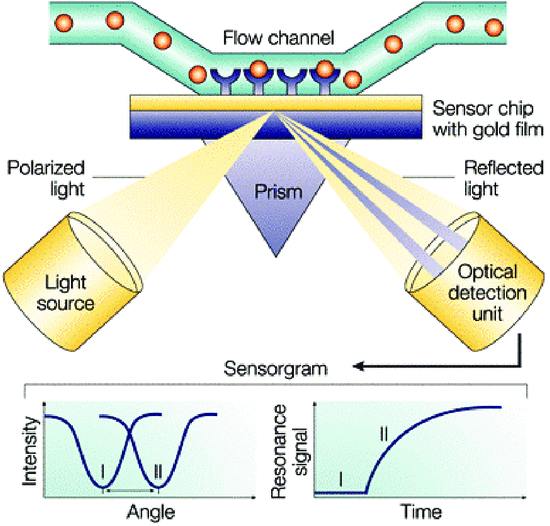
\includegraphics[width=.9\columnwidth]{Optical_SPR}
\end{minipage}\vspace{\boxmargin}
\begin{minipage}{.7\columnwidth-\boxmargin}
    \textbf{Launch a SPP}:
    \quad $0\leq k_{\vert\vert,\textrm{inc}} \leq k_0\;n\ped{inc}$\\
    must ensure \highlight{$\beta \overset{!}{=} k_{\vert\vert,\textrm{inc}} = k_0\;n\ped{inc}\;\sin\theta$}
    \quad $\theta\in[0,\frac{\pi}{2}]$

    $\implies$ \fbox{$n\ped{inc} \geq n\sqrt{\frac{\epsilon_m}{\epsilon_m+n_c^2}}$} \fbox{$\frac{\Delta\theta}{\Delta N} \hat= \pderiv{\theta}{N} = \frac{1}{n\ped{inc}\cos\theta} \simeq \frac{1}{n\ped{inc}}$}
\end{minipage}
%%%%%%%%%%%%%%%%%%%%%%%%%%%%%%%%%%%%%%%%%%%%%%%%%%%%%%
\subsubsection{OWLS \textnormal{-- Optical Waveguide Lightmode Spectroscopy}}
%
\begin{minipage}{.5\columnwidth}
    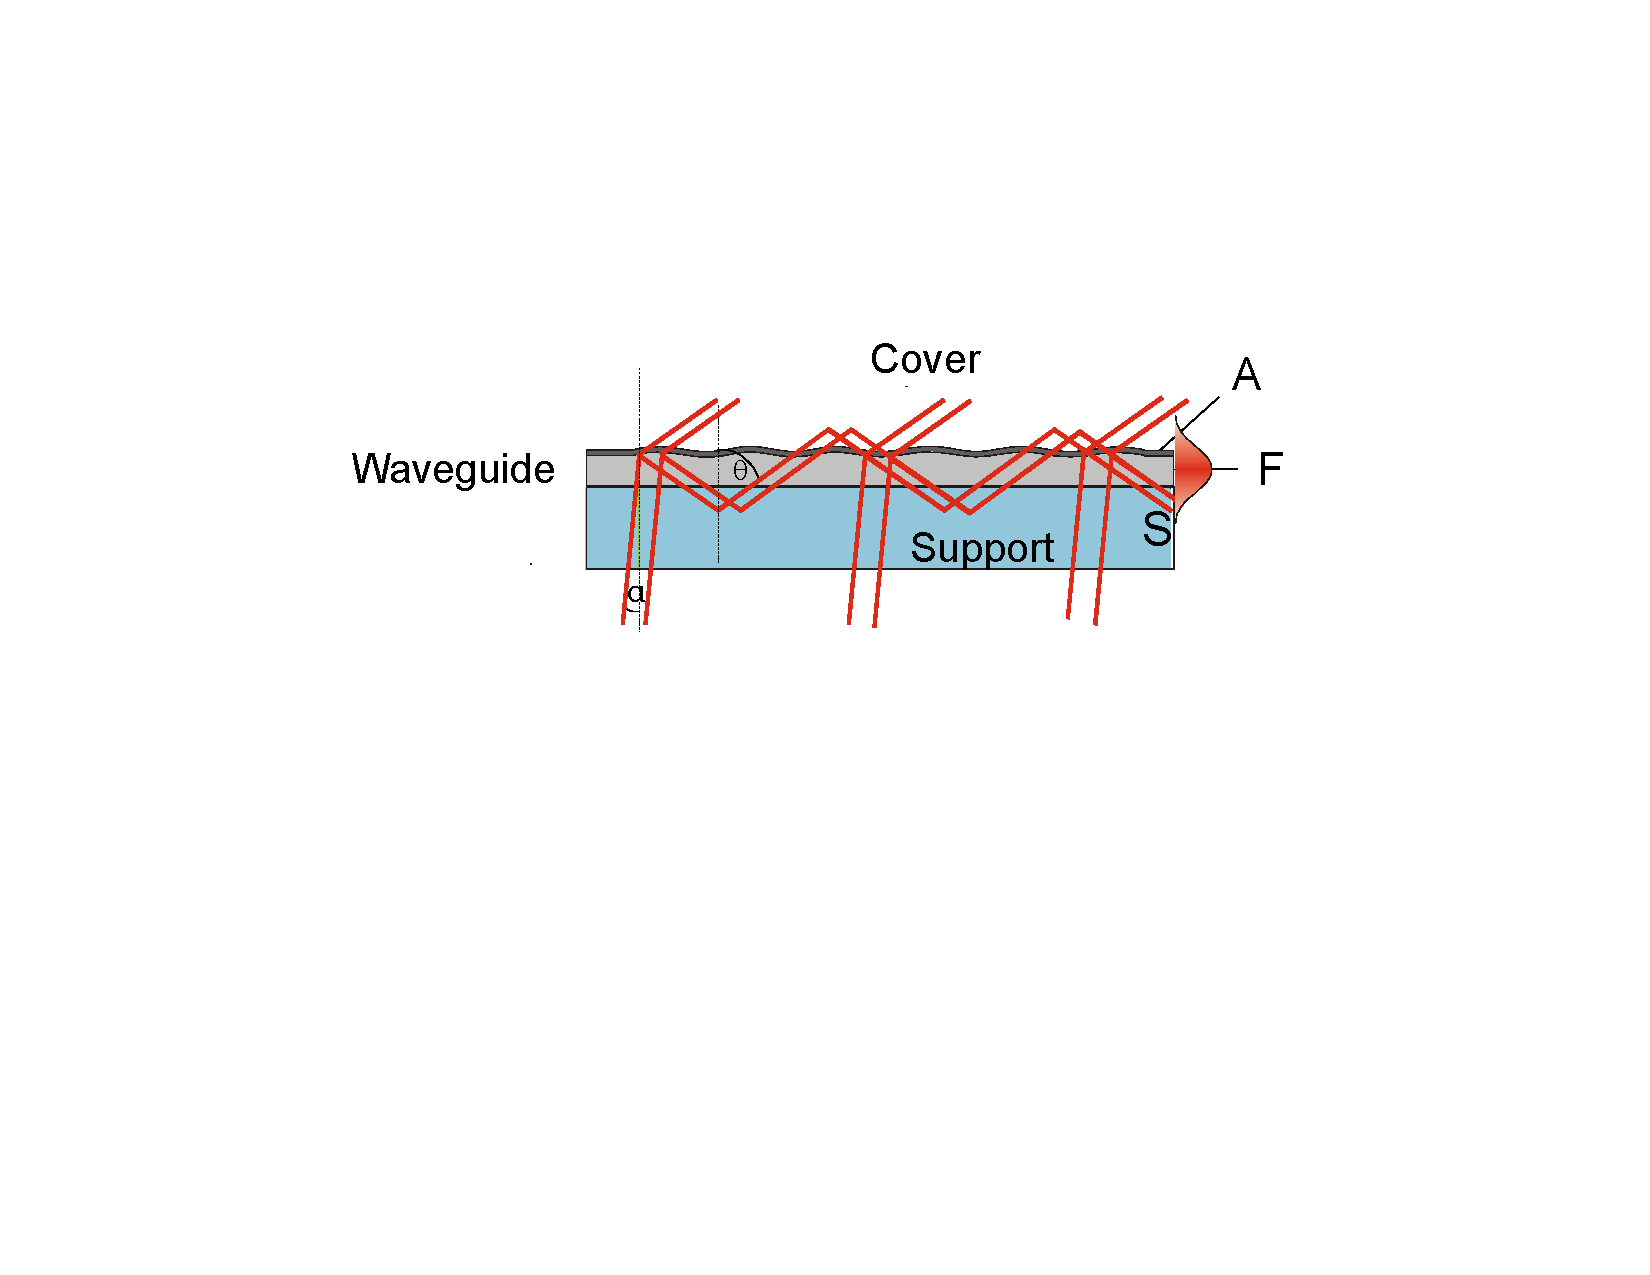
\includegraphics[width=.9\columnwidth]{Optical_OWLS}
\end{minipage}%
\begin{minipage}{.5\columnwidth}
    $N \coloneqq n_F\sin\theta = n\ped{air}\sin\alpha + \frac{l\lambda}{\Lambda}$
    \vspace{2mm}\par
    Penetr. depth \quad \fbox{$\sigma \sim \frac{\lambda}{2\pi} \frac{1}{\sqrt{N^2-n_c^2}}$}
\end{minipage}

Waves have to be in phase (constr. interf.) $\to$ extremely sensitive

\formula{constr. interference}{\textcolor{gray}{0=}\;2\pi m \overset{!}{=} \phi_F + \phi_{FS} + \phi_{FAC}}
\quad $\phi$: phase shifts

\formula{Ansatz for \textit{3 layer model}}{\scriptsize
    \begin{cases}
        \text{Cover:}		& C \;\eu^{-\abs{k_{z,C}} \;(z-d_F/2)}\\
        \text{Waveguide:}	& B \;\eu^{\iu k_{z,F} z} + A \;\eu^{\iu k_{z,F} z}\\
        \text{Support:}	& D \;\eu^{\abs{k_{z,S}} \;(z+d_F/2)}
    \end{cases}
}

\formula{Idealized adlayer}{n_A = n_C + c_A\deriv{n}{c}}
\formbox{Mass calculation}{M = \diff_A \frac{n_A-n_C}{\diff n/\diff c}}
%%%%%%%%%%%%%%%%%%%%%%%%%%%%%%%%%%%%%%%%%%%%%%%%%%%%%%
\subsection{Limitations}
%
%	Above methods are \textit{not usable for diagnostic purposes}.\\
%	For analyzing \textit{simple things} it is extremely accurate, but when the composition of the probe gets more complex (e.g. blood) your device is not usable.\\
%	However, because of the NSB problems, we cannot use it (see LOD).
Above methods not usable for \textit{diagnostic purpose} $\to$ NSB, LOD

\textbf{Solution}: diffractometric biosensors (Focal Molography)
